\documentclass[10pt,a4paper]{article}

\usepackage[T1]{fontenc}
\usepackage[utf8]{inputenc}
\usepackage{lmodern}
\usepackage[margin=2.3cm]{geometry}
\usepackage{amsmath,amssymb}
\usepackage{graphicx}
\usepackage{booktabs}
\usepackage{array}
\usepackage{url}
\usepackage{xcolor}
\usepackage{microtype}
\usepackage[hidelinks]{hyperref}
\usepackage{orcidlink}
\usepackage{caption}
\captionsetup{font=small,labelfont=bf}
\setlength{\parskip}{0.4em}
\setlength{\parindent}{0pt}

\graphicspath{{../figures/}}
% Generated by data/measure.py from beyond.json. Do not edit.
\newcommand{\nSeedsOne}{5}
\newcommand{\nSeedsOneFull}{3}
\newcommand{\sigmaBOne}{0.145}
\newcommand{\sigmaBOneMax}{0.240}
\newcommand{\sigmaMsevenThirty}{5.19}
\newcommand{\sigmaMsevenHundred}{5.20}
\newcommand{\sigmaNoModel}{5.23}
\newcommand{\sigmaMfour}{18.7}
\newcommand{\sigmaMsix}{5.4}
\newcommand{\sigmaMsevenIdeal}{0.028}
\newcommand{\costXtalk}{186}
\newcommand{\sigmaBOneIdeal}{5.27}
\newcommand{\ratioOneMed}{33}
\newcommand{\ratioOneMin}{22}
\newcommand{\ratioOneMax}{60}
\newcommand{\effBOne}{0.743}
\newcommand{\effMseven}{0.747}
\newcommand{\effRatioOne}{0.994}
\newcommand{\effRatioOneMin}{0.993}
\newcommand{\parLambda}{850}
\newcommand{\parFocal}{250}
\newcommand{\parPitch}{12.5}
\newcommand{\parNpix}{256}
\newcommand{\parPad}{2}
\newcommand{\parNa}{0.5}
\newcommand{\parXtSigma}{1.24}
\newcommand{\parXtQ}{1.80}
\newcommand{\parUp}{3}
\newcommand{\parBits}{4}
\newcommand{\parFill}{0.85}
\newcommand{\parCgSteps}{3}
\newcommand{\parWarm}{12}
\newcommand{\parOuter}{4}
\newcommand{\parFrames}{13}
\newcommand{\parFrameIters}{10}
\newcommand{\parPhaseVel}{0.3}
\newcommand{\parSubsteps}{10}
\newcommand{\parColdIters}{30}
\newcommand{\parBaseIters}{30 and 100}
\newcommand{\seedOneSigmaB}{0.0911}
\newcommand{\seedOneSigmaM}{4.454}
\newcommand{\seedOneRatio}{49}
\newcommand{\seedOneEffB}{0.7423}
\newcommand{\seedOneEffM}{0.7447}
\newcommand{\sigmaBOneFull}{0.67}
\newcommand{\sigmaMsevenFull}{5.74}
\newcommand{\sigmaNoModelFull}{5.58}
\newcommand{\ratioOneFullMed}{8.3}
\newcommand{\ratioOneFullMin}{6.9}
\newcommand{\ratioOneFullMax}{10.5}
\newcommand{\effRatioOneFull}{0.989}
\newcommand{\bakeCeightBOneSigma}{6.71}
\newcommand{\bakeCeightMsevenSigma}{14.76}
\newcommand{\bakeCeightRatio}{2.2}
\newcommand{\bakeCeightBOneEff}{0.648}
\newcommand{\bakeCeightMsevenEff}{0.675}
\newcommand{\bakeCeightEffRatio}{0.960}
\newcommand{\bakeCeightIters}{30}
\newcommand{\bakeCeightTraps}{64}
\newcommand{\bakeCeightPix}{128}
\newcommand{\nSeedsTwo}{5}
\newcommand{\bTwoMin}{0.918}
\newcommand{\bTwoMed}{0.920}
\newcommand{\bTwoMax}{0.925}
\newcommand{\lpiMin}{0.536}
\newcommand{\lpiMed}{0.656}
\newcommand{\lpiMax}{0.724}
\newcommand{\bTwoSigmaFrame}{0.41}
\newcommand{\lpiSigmaFrameMin}{18}
\newcommand{\lpiSigmaFrameMax}{29}
\newcommand{\bTwoMedSeven}{0.752}
\newcommand{\bTwoMinSeven}{0.734}
\newcommand{\lpiMedSeven}{0.646}
\newcommand{\lpiMaxSeven}{0.687}
\newcommand{\bTwoMedTwentyFive}{0.969}
\newcommand{\bTwoMinTwentyFive}{0.965}
\newcommand{\lpiMedTwentyFive}{0.657}
\newcommand{\lpiMaxTwentyFive}{0.739}


% Page-1 header block (conventions/manuscript-header-standard.md). The four document macros are set by the
% publishing tool when the version DOI is reserved.
\newcommand{\doctype}{Preprint}
\newcommand{\docversion}{v0.01}
\newcommand{\docdate}{30 October 2026}
\newcommand{\versiondoi}{10.5281/zenodo.23788734}
\newcommand{\conceptdoi}{10.5281/zenodo.23788733}
\newcommand{\docrepo}{github.com/fsantibanezleal/CEFOP\_DinHot}
\newcommand{\headerblock}{%
\begin{center}
\fbox{\parbox{0.94\textwidth}{\small\raggedright
\textbf{\doctype} \quad$\cdot$\quad \docversion, \docdate \quad$\cdot$\quad Licence CC BY 4.0\\[2pt]
CAOS open-research programme \quad$\cdot$\quad CEFOP\_DinHot, holographic optical trap studio, claims BS-1 and BS-2\\[2pt]
Version DOI \href{https://doi.org/\versiondoi}{\texttt{\versiondoi}} \quad$\cdot$\quad
concept DOI (always latest) \href{https://doi.org/\conceptdoi}{\texttt{\conceptdoi}}\\[2pt]
Not peer reviewed. Source code, data and computational records: \href{https://\docrepo}{\texttt{\docrepo}}
}}
\end{center}
\vspace{4pt}}

\begin{document}

\title{Device-Aware Weighted Gerchberg--Saxton and Flicker-Bounded Phase-Continuous Sequences\\ for Holographic Optical Trap Arrays}
\author{Felipe Santib\'a\~nez-Leal~\orcidlink{0000-0002-0150-3246}\\
\small CAOS open-research programme, Santiago, Chile\\
\small \texttt{fsantibanez@gmail.com}}
\date{}
\maketitle
\vspace{-1.2em}
\headerblock

\begin{abstract}
Phase-fixed weighted Gerchberg--Saxton (WGS) is the practical state of the art for large arrays of optical traps, but it
optimizes the hologram on an ideal model of the spatial light modulator (SLM), and the sequences that move traps interpolate
between holograms that were never optimized for the frames in between. We test two hypotheses against the strongest baselines
on the same scalar Fourier model. First, keeping the WGS weights but replacing the phase update by conjugate-gradient steps through the
pixel-crosstalk kernel and the phase quantizer of the device (device-aware WGS) lowers the trap-intensity spread on the device. On a
$10\times10$ lattice behind a crosstalk device, the relative standard deviation falls from a median of \sigmaMsevenThirty{} percent for phase-fixed
WGS at 30 iterations (\sigmaMsevenHundred{} percent at 100) to \sigmaBOne{} percent, a median factor of \ratioOneMed{} over
\nSeedsOne{} seeds (range \ratioOneMin{} to \ratioOneMax) at a median \effRatioOne{} of the baseline's efficiency; the factor is \ratioOneFullMed{} with \parBits{}-bit
phase and a fill factor of \parFill{} added, and \bakeCeightRatio{} on a smaller $8\times8$ grid with a fixed \bakeCeightIters{}-iteration budget; over the \benchOneDevN{} geometries
of the studio's benchmark on its full device the median factor is \benchOneDevMed{} (\benchOneDevMin{} to \benchOneDevMax), and \benchOneDevPass{} of
them meet both thresholds. A control that removes the device model from the loop gains nothing
(\sigmaNoModel{} percent), so the gain comes from the model. Second, optimizing every intermediate hologram of a moving-trap sequence with the trap phases locked to a smooth
trajectory (flicker-bounded sequence) keeps the minimum transient intensity of the moving traps at a median \bTwoMed{} of their mean (range \bTwoMin{} to \bTwoMax) over \nSeedsTwo{} seeds at thirteen frames (below $0.9$ at seven frames),
against \lpiMed{} (\lpiMin{} to \lpiMax) for linear phase interpolation. The bound holds while the peak step per frame is at most \claimStepFu{} Fourier units: on longer
lattice moves it is met on \longAMet{} and \longBMet{} of \longSeeds{} seeds with the frames that step implies, and on the long sort of a rearrangement case linear phase
interpolation leads at an equal number of frames. Both results hold in a model of a simulated device and in a transient model that we define; neither is a
hardware measurement.
\end{abstract}

\noindent\textbf{Keywords:} holographic optical tweezers, weighted Gerchberg--Saxton, pixel crosstalk, phase quantization, linear phase interpolation, atom rearrangement.

\section{Introduction}

A phase-only SLM in the pupil plane of a lens forms an array of optical traps whose number reaches thousands. The hologram that does it is computed, not designed, and
three families of method dominate large arrays. The Gerchberg--Saxton (GS) iteration and its weighted form~\cite{dileonardo} equalize the trap intensities in the ideal model;
freezing the focal-plane phase after a few iterations (phase-fixed WGS)~\cite{kim2019} keeps the weights effective and reaches percent-level uniformity on arrays of 1500
foci, and the same algorithm computes the holograms of the 256-atom and 6100-atom arrays~\cite{ebadi,manetsch}. Camera feedback then corrects the residual spread on the experiment~\cite{nogrette,kim2019}.
Gradient methods with a device model exist for shaped potentials~\cite{schroff}, and a convolution of the phase inside a weighted GS has been used to reduce crosstalk
while replacing amplitudes only~\cite{persson}.

Two gaps follow. (i) The solver of the large-array methods has no model of the device. The pixel crosstalk, the phase quantization and the finite fill factor of a real SLM
change the trap intensities after the hologram is computed, and the experiments absorb the change with camera iterations. A model of crosstalk was placed in
conjugate-gradient minimization of shaped potentials~\cite{schroff}, but not inside a weighted GS for point traps. (ii) The sequences that rearrange atoms with an SLM
interpolate the position, the amplitude and the optical phase of every trap between two endpoint holograms and invert the transform at every step~\cite{lpi};
the intermediate holograms are never individually optimized, their trap intensities are uneven, and the interference of the transient spots makes the intensity dip.

We propose and test a method for each gap. Section~\ref{sec:model} fixes the model, Section~\ref{sec:b1} defines the device-aware WGS (BS-1) and
Section~\ref{sec:b2} the flicker-bounded sequence (BS-2), each with the hypothesis that would refute it, the baseline, the protocol and the results.
Section~\ref{sec:limits} states what the results do not show.

\section{Model and metrics}\label{sec:model}

The SLM has $n_{\mathrm{pix}}\times n_{\mathrm{pix}}$ pixels of pitch $p$ and a Gaussian input beam normalised so that $\sum_jA_j^2=n_{\mathrm{pix}}^2$. For a trap $m$ at $(x_m,y_m)$ in the focal plane of a lens of
focal length $f$ at wavelength $\lambda$, the field and the intensity are
\begin{equation}
V_m=\frac1{n_{\mathrm{pix}}^2}\sum_jA_je^{\,i(\phi_j-\Delta_j^m)},\qquad \Delta_j^m=\frac{2\pi}{\lambda f}(x_jx_m+y_jy_m),\qquad I_m=|V_m|^2,
\end{equation}
following Di Leonardo et al.~\cite{dileonardo}, and equal to the entries of the zero-padded FFT of the SLM field for traps on FFT bins. The efficiency is $e=\sum_mI_m$ and the
spread is the relative standard deviation $\sigma=100\operatorname{std}(I)/\operatorname{mean}(I)$ in percent, with $I$ divided by the target weights.

\textbf{Device.} The displayed phase is wrapped, quantized to $2^b$ levels and blurred. Each SLM pixel is $u\times u$ computational pixels ($u=\parUp$) and the phase is convolved with the kernel
\begin{equation}
K=\mathcal F^{-1}\Big\{\exp\Big[-\frac{|k_x|^q+|k_y|^q}{\sigma_K^q}\Big]\Big\},\qquad \sigma_K=\parXtSigma,\ q=\parXtQ,
\end{equation}
the fitted values of Schroff et al.~\cite{schroff}. The focal field of what the device displays is the FFT of the blurred, upsampled phase on the finer grid, cropped to the
same window, times the field envelope of a square pixel of fill factor $\mathrm{fill}$. The adjoint of the blur (convolution with the reversed kernel and a sum over each $u\times u$ block) is closed form.
Two devices are used: the \emph{crosstalk device} (the kernel above, no quantization, fill factor one) and the \emph{full device} (the kernel, \parBits{}-bit phase and a fill factor of \parFill; random flicker is not applied).
Every hologram is scored on the device with the same function, whatever model it was optimized on.

\textbf{Task and setup.} The task is a $10\times10$ square lattice of equal traps eight FFT bins apart on an SLM of $\parNpix^2$ pixels padded by \parPad, with $\lambda=\parLambda$~nm, $f=\parFocal$~mm, $p=\parPitch$~$\mu$m and
NA $\parNa$ in air. All methods are deterministic given a seed.

\section{BS-1: device-aware weighted GS}\label{sec:b1}

\subsection{Hypothesis and method}

\emph{Hypothesis.} If the crosstalk kernel and the quantizer are inside the weighted GS loop, the trap intensities on the device are at least twice as uniform as those of phase-fixed WGS,
which optimizes on the ideal model, at an efficiency no more than ten percent lower. The hypothesis is refuted if the factor is below two or the efficiency drops by more than ten percent.

\emph{Method.} Keep the weight update of weighted GS, $w_m\leftarrow w_m\langle r\rangle/r_m$ with $r_m=|V_m|/a_m$ the trap amplitude relative to its design amplitude~\cite{dileonardo}, but measure $r_m$ on the
device's focal field, and replace the projection of the phase update by $K_{\mathrm{cg}}=\parCgSteps$ conjugate-gradient steps on the device-aware loss
\begin{equation}
L(\phi)=\frac{\sum_m\big(|V_m(\phi)|^2-T_m\big)^2}{\sum_mT_m^2},\qquad T_m=\eta\,\frac{(w_ma_m)^2}{\sum_k(w_ka_k)^2},\qquad \eta=\sum_m|V_m|^2,
\end{equation}
where $V=\mathrm{Op}(\phi)$ runs through the straight-through quantizer, the crosstalk operator, the FFT of the upsampled grid and the pixel envelope. The target level is the current efficiency $\eta$, so the steps flatten the traps without
trading efficiency away; the weights supply the integral feedback that few steps per iteration lack. The gradient is the closed form through the crosstalk adjoint, so no automatic differentiation is needed.
The conjugate-gradient steps are Fletcher--Reeves with a strong-Wolfe line search, restarted at every outer iteration because the target changes with the weights. The start is \parWarm{} iterations of weighted GS on the ideal model,
and there are \parOuter{} outer iterations. The weight update is an integrator that a few gradient steps may not follow on a device they
cannot fit, so B1 returns its best iterate, the warm start included: the phase of lowest spread on its device model among the iterates that keep
at least \parFloor{} of the warm start's efficiency, the bound of the hypothesis. A run whose weights wind up therefore never returns worse than its start.

\subsection{Baselines and protocol}

The strongest baseline is phase-fixed WGS (M07)~\cite{kim2019}, run on the ideal model for \parBaseIters{} iterations and scored on the device; the lower spread of the two runs is the reference, because more iterations cannot remove a
crosstalk the model does not contain. Plain GS (M04) and weighted GS (M06) at 30 iterations are reported for context. As a control, the same B1 loop is run with the device model removed (the ideal model in the loop), and scored on the device.
Each configuration runs on \nSeedsOne{} seeds; the full device runs on \nSeedsOneFull{}.

\subsection{Results}

\begin{table}[t]
\centering\small
\caption{BS-1 on the $10\times10$ task, scored on the device. Medians over the seeds; $\sigma$ is the relative standard deviation of the trap intensities (\%), $e$ the efficiency.}
\label{tab:b1}
\begin{tabular}{@{}l r r r@{}}
\toprule
Method & $\sigma$ on the crosstalk device & $\sigma$ on the full device & $e$ (crosstalk device)\\
\midrule
GS (M04), 30 iterations & \sigmaMfour & n/a & n/a\\
Weighted GS (M06), 30 iterations & \sigmaMsix & n/a & n/a\\
Phase-fixed WGS (M07), 30 iterations & \sigmaMsevenThirty & \sigmaMsevenFull & \effMseven\\
Phase-fixed WGS (M07), 100 iterations & \sigmaMsevenHundred & n/a & n/a\\
B1 with the device model removed & \sigmaNoModel & \sigmaNoModelFull & n/a\\
B1 (device-aware WGS) & \sigmaBOne & \sigmaBOneFull & \effBOne\\
\bottomrule
\end{tabular}
\end{table}

Table~\ref{tab:b1} and Fig.~\ref{fig:b1} give the result. On the crosstalk device, phase-fixed WGS leaves a spread of \sigmaMsevenThirty{} percent at 30 iterations and \sigmaMsevenHundred{} percent at 100 although it
reaches \sigmaMsevenIdeal{} percent on the ideal model: the crosstalk costs a factor of about \costXtalk{}. B1 reduces the spread to a median of \sigmaBOne{} percent (largest value \sigmaBOneMax{} percent), a median factor of
\ratioOneMed{} (range \ratioOneMin{} to \ratioOneMax) against the better of the two baseline runs, at a median \effRatioOne{} of the baseline's efficiency (smallest ratio \effRatioOneMin). The factor varies from seed to seed with the baseline's own spread, so the distribution, not one seed, is the result (Fig.~\ref{fig:b1}b). The control that keeps B1's structure but removes the device model from the loop stays at \sigmaNoModel{} percent, the level of the baseline, so the gain comes from the device model and
not from the extra iterations or the gradient steps. B1 pays for this on the ideal model: scored without the device, its spread is \sigmaBOneIdeal{} percent, because its hologram is built to cancel the crosstalk, not to be uniform before it.

With \parBits{}-bit phase and a fill factor of \parFill{} added, the baseline spread is \sigmaMsevenFull{} percent and B1 reaches \sigmaBOneFull{} percent, a median factor of \ratioOneFullMed{} (range \ratioOneFullMin{} to \ratioOneFullMax) at \effRatioOneFull{} of the efficiency; the model-free control stays at \sigmaNoModelFull{} percent.
On the small $8\times8$ array on a $\bakeCeightPix^2$-pixel SLM with the same four effects and a fixed budget of \bakeCeightIters{} iterations (the device-limited case of the studio), the baked scores are \bakeCeightBOneSigma{} percent for B1 and
\bakeCeightMsevenSigma{} percent for M07, a factor of \bakeCeightRatio{}, with an efficiency ratio of \bakeCeightEffRatio. The factor is therefore not a constant: it depends on the grid, the device and the budget, and on the seed (Fig.~\ref{fig:b1}b).

\begin{figure}[t]
\centering
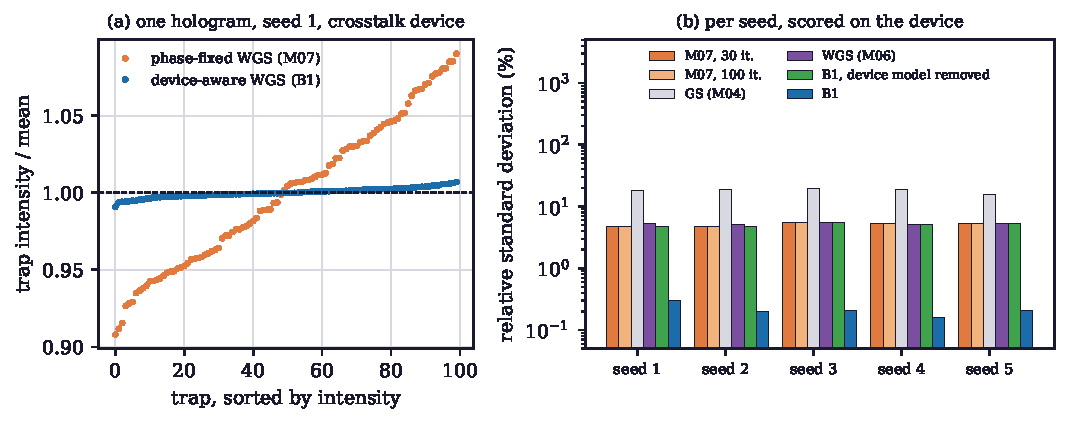
\includegraphics[width=\textwidth]{fig-b1.pdf}
\caption{BS-1. (a) Sorted trap intensities of one hologram (seed 1) on the crosstalk device: phase-fixed WGS leaves a spread, B1 is flat. (b) Relative standard deviation on the device for every seed (log scale): the baselines, B1 with the device
model removed from the loop, and B1.}
\label{fig:b1}
\end{figure}

\section{BS-2: flicker-bounded phase-continuous sequences}\label{sec:b2}

\subsection{Hypothesis and method}

\emph{Hypothesis.} If every frame of a sequence is optimized with the optical phases of the traps locked to a smooth trajectory, a moving trap never drops below $0.9$ of its mean intensity, where interpolating independent
endpoint holograms does not achieve it. The hypothesis is refuted if the minimum transient ratio is below $0.9$ or not above that of linear phase interpolation (LPI).

\emph{Method.} Positions follow the minimal-jerk profile $x_m(s)=x_m(0)+(x_m(S)-x_m(0))(10\tau^3-15\tau^4+6\tau^5)$, $\tau=s/S$. The phases are $\theta_m(s)=\theta_m(0)+\operatorname{wrap}(\theta_m^{\mathrm{end}}-\theta_m(0))h(\tau)$ with the same profile $h$
(default: phases held), and the sequence is refused if the phase step per frame exceeds \parPhaseVel{} rad. Each frame is a phase-fixed WGS step with the trap phases locked,
\begin{equation}
c_m=w_ma_me^{i\theta_m(s)},\qquad w_m\leftarrow w_m\langle r\rangle/r_m,\qquad \phi_j=\arg\sum_mc_me^{+i\Delta_j^m(x_m(s))},
\end{equation}
started from the previous frame's hologram and weights and run for \parFrameIters{} iterations; frame 0 is a cold phase-fixed WGS of \parColdIters{} iterations. The hard lock is the limit of a penalty on the phase deviation. The default sequence has \parFrames{} frames.

\emph{Transient intensity.} Between frames $s$ and $s+1$ the displayed field is modelled as the blend $f_a=A[(1-a)e^{i\phi_s}+ae^{i\phi_{s+1}}]$, $a\in[0,1]$ (\parSubsteps{} sub-frames), and trap $m$ is read at its trajectory point $x_m(s+a)$, giving $I_m(s,a)=|V_m(f_a;x_m(s+a))|^2$. The
transient ratio of a trap is $\min_{s,a}I_m(s,a)/\operatorname{mean}_sI_m(s)$. This blend model is our own; the source of the baseline gives a measurement, not an equation, so the absolute ratios are properties of the model and are compared between methods only.

\subsection{Baseline and protocol}

LPI follows the published description~\cite{lpi}: two independently computed endpoint holograms (phase-fixed WGS, \parColdIters{} iterations), each trap's position, amplitude and optical phase read from them, linearly interpolated over the same frames (the phase by its wrapped
difference), and the transform inverted at every frame (the superposition of the interpolated spots, no per-frame optimization). Both sequences are scored by the same function. The task is a $4\times4$ lattice eight bins apart in which the two right-hand columns, eight traps, move four bins. Each condition runs on \nSeedsTwo{} seeds.

\subsection{Results}

\begin{figure}[t]
\centering
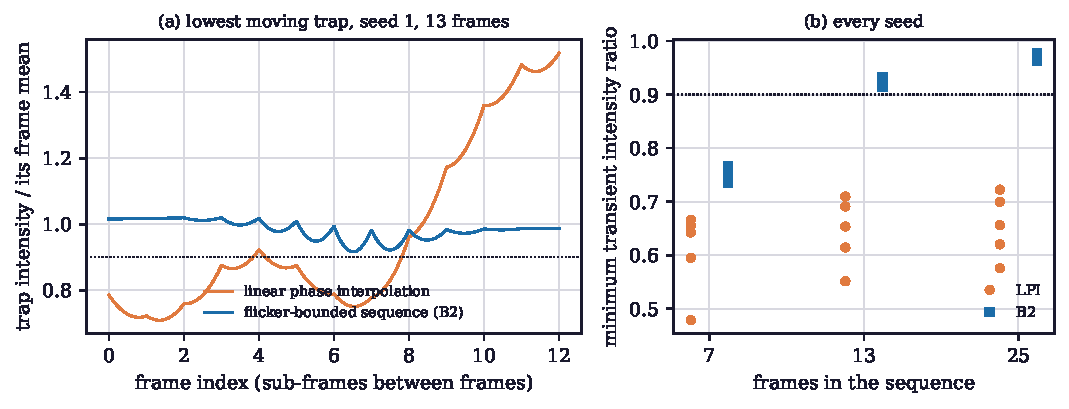
\includegraphics[width=\textwidth]{fig-b2.pdf}
\caption{BS-2. (a) Intensity of the moving trap with the lowest minimum, divided by its frame mean, along the 13-frame sequence (seed 1): LPI dips and overshoots, the flicker-bounded sequence stays close to one. The dotted line is $0.9$. (b) Minimum transient ratio of the moving traps against the length of the sequence, one marker per seed.}
\label{fig:b2}
\end{figure}

With \parFrames{} frames the minimum transient ratio of the moving traps is a median \bTwoMed{} (range \bTwoMin{} to \bTwoMax) for the flicker-bounded sequence, above $0.9$ for every seed, against \lpiMed{} (\lpiMin{} to \lpiMax) for LPI, which is below $0.9$ for every seed. The
per-frame uniformity differs by two orders: the largest per-frame relative standard deviation is at most \bTwoSigmaFrame{} percent for the flicker-bounded sequence and between \lpiSigmaFrameMin{} and \lpiSigmaFrameMax{} percent for LPI, because the intermediate frames of LPI are not optimized. Fig.~\ref{fig:b2}a shows the
trajectory of the worst trap. With seven frames the bound of $0.9$ is not met: the medians are \bTwoMedSeven{} (B2, smallest \bTwoMinSeven) and \lpiMedSeven{} (LPI, largest \lpiMaxSeven), so B2 stays above LPI but the hypothesis as stated is refuted at that length, where each frame moves the traps farther. With twenty-five frames the medians are \bTwoMedTwentyFive{} (B2) and \lpiMedTwentyFive{} (LPI); the smallest value of B2 is \bTwoMinTwentyFive{} and the largest value of LPI \lpiMaxTwentyFive{} (Fig.~\ref{fig:b2}b).

\subsection{Scope: long moves}\label{sec:b2scope}

The task above moves the traps four bins in thirteen frames. The method names the fewest frames whose peak step under the minimal-jerk profile is at most
\claimStepFu{} Fourier units, and the scope of the claim is measured on longer moves with the end phases taken from phase-fixed WGS at the destination. On the same
lattice with the two columns moved \longABins{} and \longBBins{} bins (\longAFu{} and \longBFu{} Fourier units, $64^2$ pixels padded by 2), the \scopeDefaultFrames{} default
frames leave the lowest moving trap at most at \longDefaultMax{} over \longSeeds{} seeds; with the \longAFrames{} and \longBFrames{} frames of the move the medians are
\longAMed{} and \longBMed{}, and \longAMet{} and \longBMet{} of the \longSeeds{} seeds reach $0.9$ (the lowest \longALow{} and \longBLow).

On the rearrangement case of the studio (C10: \cTenTraps{} target sites, \cTenMoving{} of them reached by a move on the assignment of the Hungarian method, the longest
\cTenFu{} Fourier units), held phases dim the moving traps to \cTenHeld{} at \cTenEqual{} frames (first seed). With the end phases at \cTenEqual{} frames, a peak step of
\cTenPeakEqual{} Fourier units, LPI on the same assignment leads on \cTenLpiLeads{} of \cTenSeeds{} seeds (B2 at most \cTenBEqualMax, LPI \cTenLEqualMin{} to \cTenLEqualMax).
With the \cTenFrames{} frames of the move, B2 reaches \cTenMetMin{} to \cTenMetMax{} (median \cTenMetMed) on \cTenMet{} of the \cTenSeeds{} seeds and leads LPI
(\cTenLpiMin{} to \cTenLpiMax) on \cTenBLeads; its lowest seed is at \cTenLowest. The claim therefore holds in the short-step regime and with the frames that regime
implies, not at an equal number of frames on long moves.

\section{Limits}\label{sec:limits}

\textbf{Model, not instrument.} Both results are computed on a scalar Fourier model with the device effects stated above. The crosstalk parameters come from a published fit on another device; the \parBits{}-bit, fill-factor and flicker effects have no published source in this model, and random flicker is not applied in the scoring. The frequency unit of the kernel is
carried over from the model and is not verified against the source. An instrument with a different kernel would give a different factor, and the sensitivity of B1 to a mismatched kernel was not tested.

\textbf{Variation.} The BS-1 factor ranges over the seeds from \ratioOneMin{} to \ratioOneMax{} on one task, and falls to \ratioOneFullMed{} on the full device and to \bakeCeightRatio{} on the smaller grid with a fixed budget. The result is a large improvement on this task, not a constant. The number of seeds is \nSeedsOne{} for the crosstalk device and \nSeedsOneFull{} for the full device; on the \benchOneDevN{} geometries of the studio's benchmark, on its C08 device (which adds flicker) at \benchOneBudget{} iterations with the
default parameters and \benchOneDevSeedsMin{} to \benchOneDevSeedsMax{} seeds per cell, the factor over phase-fixed WGS has a median of \benchOneDevMed{}
(\benchOneDevMin{} to \benchOneDevMax) at a median efficiency ratio of \benchOneDevEff, and \benchOneDevPass{} of them meet both thresholds of the hypothesis:
the gain is that of the task and devices above, and it does not carry to every geometry.
B1 is built for traps on FFT bins at the focal plane without vortices, and is more expensive than the baseline by about the square of the upsampling factor per step; it is a baked method, not a live one.

\textbf{BS-2 transient model.} The ratio of BS-2 is defined by our blend model of the SLM field between frames. It omits the temporal response and the refresh of the device, and the LPI baseline is our implementation of a published description, not the authors' code. In the source of the baseline, LPI on hardware stays above $0.70$ of its intensity, whereas it scores lower here
under our model, so the absolute values are not comparable between the two. The result establishes the ordering of the two methods under one model, on the acceptance task and, within the step bound, on the longer moves of Section~\ref{sec:b2scope};
at an equal number of frames on a long sort, LPI leads. It does not show that atoms are rearranged with fewer losses.

\textbf{What is not claimed.} Neither method is shown to improve a camera-corrected experiment. B1 is not compared with conjugate gradient on the same point-trap task, whose gradient-based shaped-potential variant needs ten minutes per hologram in its source~\cite{schroff}.

\section{Conclusion}

Putting the pixel-crosstalk kernel and the phase quantizer inside the weighted GS loop lowers the trap-intensity spread on the device by a median factor of \ratioOneMed{} on a $10\times10$ lattice at \effRatioOne{} of the baseline efficiency, and the gain disappears when the device model is removed from the loop. Optimizing each intermediate frame with locked, smoothly varying trap phases keeps moving traps above \bTwoMin{} of their mean
intensity at thirteen frames or more (but not at seven) where linear phase interpolation falls to \lpiMed{}, as long as the peak step per frame is at most
\claimStepFu{} Fourier units; a long move needs the frames that bound implies, and at an equal number of frames on a long sort LPI leads. Both are demonstrated in simulation with the limits above; the experiments that would confirm or refute them need the camera-in-the-loop measurement on an SLM with a fitted device model.

\section*{Data and code availability}

The methods (B1 and B2), the baselines, the measurement script that regenerates every number, table and figure reported here (\texttt{manuscripts/device-aware-flicker-bounded/data/measure.py}) and the committed baked artifacts it reads are in the repository
\url{https://github.com/fsantibanezleal/CEFOP_DinHot} (Apache-2.0). The studio runs at \url{https://dinhot.fasl-work.com}. The acceptance tests of the two methods are \texttt{tests/methods/beyond/test\_b1\_device\_wgs.py} and \texttt{test\_b2\_flicker\_bounded.py}.

\begin{thebibliography}{99}\small
\bibitem{dileonardo} Di Leonardo, Ianni and Ruocco, ``Computer generation of optimal holograms for optical trap arrays,'' \emph{Opt. Express} 15, 1913, 2007. doi:10.1364/OE.15.001913.
\bibitem{kim2019} Kim, Kim, Lee and Ahn, ``Large-scale uniform optical focus array generation with a phase spatial light modulator,'' \emph{Opt. Lett.} 44, 3178, 2019. doi:10.1364/OL.44.003178.
\bibitem{ebadi} Ebadi \emph{et al.}, ``Quantum phases of matter on a 256-atom programmable quantum simulator,'' arXiv:2012.12281, 2021.
\bibitem{manetsch} Manetsch \emph{et al.}, ``A tweezer array with 6100 highly coherent atomic qubits,'' \emph{Nature} 647, 60--67, 2025. arXiv:2403.12021.
\bibitem{nogrette} Nogrette \emph{et al.}, ``Single-atom trapping in holographic 2D arrays of microtraps with arbitrary geometries,'' arXiv:1402.5329, 2014.
\bibitem{schroff} Schroff, La Rooij, Haller and Kuhr, ``Accurate holographic light potentials using pixel crosstalk modelling,'' \emph{Sci. Rep.}, 2023. doi:10.1038/s41598-023-30296-6.
\bibitem{persson} Persson, Engstr\"om and Goks\"or, ``Reducing the effect of pixel crosstalk in phase only spatial light modulators,'' \emph{Opt. Express} 20, 22334, 2012.
\bibitem{lpi} ``Parallel assembly of neutral atom arrays with an SLM using linear phase interpolation,'' arXiv:2501.01391.
\end{thebibliography}

\end{document}
